\documentclass[a4paper]{report}
\usepackage{graphicx}
\usepackage{booktabs}

\title{Foreign Exchange Management System (FXMS)}
\author{
    Yazeed AlKhalaf \\
    Mohammed Bin Jebreen \\
    Nawaf AlAmer \\
    \textbf{Course:} SWE 301 - Requirements Engineering \\
    \textbf{Instructor:} Dr. Noureddine Abbadeni
}
\date{20 Feb, 2024}

\begin{document}

\maketitle

\newpage

\tableofcontents

\chapter{System Request (FXMS)}

\section{Project Sponsor}
Dr. Noureddine Abbadeni

\section{Business Need}
The need for a project like the Foreign Exchange Management System (FXMS) is crucial for businesses operating internationally for several reasons:
\begin{itemize}
    \item \textbf{Operating internationally:} Businesses engaged in importing and exporting goods and services will need a system like FXMS for currency conversion, enabling them to exchange their local currency for that of the country in which they wish to operate, thereby settling international transactions.
    \item \textbf{Managing cash flow:} Businesses operating overseas need to manage their cash across multiple currencies. FXMS will help them monitor and optimize their cash by converting currency at favorable rates and timings.
    \item \textbf{Softening the risk:} FXMS will provide businesses with tools to manage and mitigate the risks associated with fluctuations in currency prices. By using specific strategies, companies can lower the risk of exchange rate volatility and protect their profit margins.
\end{itemize}

\section{Business Requirements}
The functionality that the system should have includes:
\begin{itemize}
    \item Ability to manage clients and accounts (insert, update, delete).
    \item Ability to manage trades (insert, update, and delete trades). Any trader can enter new trades while updating and deleting existing trades require specific privileges.
    \item Ability to manage traders and coverage groups by assigning a trader to a coverage group, moving a trader from one coverage group to another.
    \item Ability to manage currencies and rates including daily updates of rates available in the market. The system is assumed to be connected with another system (such as Tadawul) which provides daily updates for exchange rates between all currencies.
    \item The system will integrate with two systems: FX trading database and FX coverage group database. These two systems are the main data sources for the system.
\end{itemize}

\section{Business Value}
The Foreign Exchange Management System (FXMS) is expected to deliver significant gains:
\begin{itemize}
    \item \textbf{Quicker and Better Decision Making:} Facilitated by the collection of multiple systems, enhancing competitive advantage in international markets.
    \item \textbf{Less Human Error:} The human factor is limited to tasks that require human interaction and not repetitive tasks that are error-prone.
    \item \textbf{More Money:} The efficient management of trades and currency conversions is expected to increase the organization's revenue.
    \item Headcount reduction by 10 traders per branch.
    \item 15\% increase in market share.
\end{itemize}

\section{Constraints}
\begin{itemize}
    \item The system should run on Windows 10.
    \item The system should be delivered by the end of the year 2028.
    \item Security and reliability must be considered during development.
\end{itemize}

\chapter{Feasibility Study}

Overall, the risk in this project compared to the gains can be considered manageable.

\section{Technical}

The technical team is confident they can build it since they built a similar system before, the knowldege they gained during that experience lowers the risk.

\begin{itemize}
    \item \textbf{Familiarity with application:} The team is familiar with building an FXMS.
    \item \textbf{Familiarity with technology:} Since the team members have a collective experience of over 50 years building complex software, we are confident they will be able to tackle the project.
    \item \textbf{Project Size:} Large project.
    \item \textbf{Compatibility:} The company wants a custom solution, so we will make sure it integrates well by analysing before we build anything and before we choose a platform.
\end{itemize}

The techincal team is confident they can build the system even though it is big. They have built a similar system before and they are familiar with the requirements and the technology.

\newpage

\section{Financial}

\subsection{Cost-Benefit Analysis}

The cashflow analysis below in Figure \ref{fig:cash-flow-analysis} is a condensed versin of the 4 years (monthly based) version of the cashflow analysis. It gives an idea on the way the project will behave financially.

\begin{figure}[h!]
    \centering
    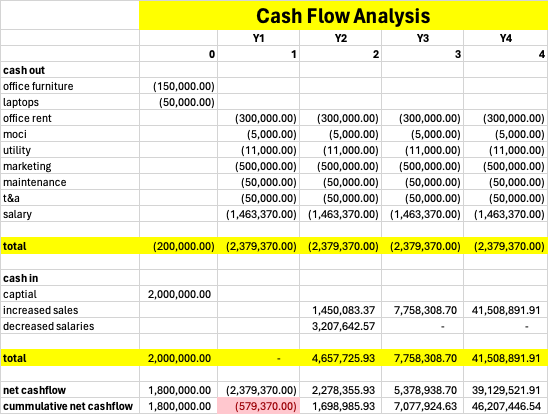
\includegraphics[width=0.8\textwidth]{images/cash-flow-analysis.png}
    \caption{Cashflow Analysis of FXMS}
    \label{fig:cash-flow-analysis}
\end{figure}

\subsection{ROI and BEP}

We will move to the big numbers, the ROI and the BEP.

\begin{figure}[h!]
    \centering
    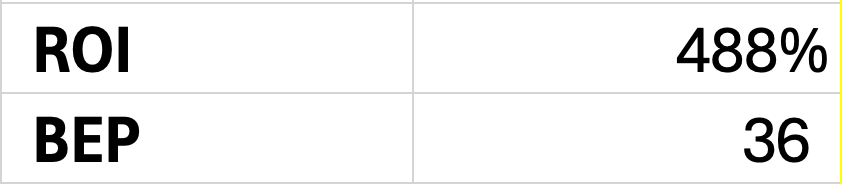
\includegraphics[width=0.8\textwidth]{images/roi-bep.png}
    \caption{ROI and BEP of FXMS}
    \label{fig:roi-and-bep}
\end{figure}

\chapter{Methodology}

Below in Table \ref{tab:methodology-criteria}, the criteria we used to choose our methodology are mentioned with what we chose. 

\begin{table}[htbp]
    \centering
    \caption{Criteria Evaluation for System Development Methodologies}
    \label{tab:methodology-criteria}
    \begin{tabular}{@{}p{0.4\linewidth}ccc@{}}
        \toprule
        Criteria & Waterfall & Parallel & V-Model \\
        \midrule
        Are the requirements clear? & Yes (Poor) & Yes (Poor) & Yes (Poor) \\
        Is the technology familiar to the team? & Yes (Poor) & Yes (Good) & Yes (Good) \\
        Is the system complex? & Yes (Good) & Yes (Good) & Yes (Good) \\
        Does the system need to be reliable? & Yes (Good) & Yes (Good) & Yes (Excellent) \\
        Is the system scheduled to be built in a short time? & No (Poor) & No (Good) & No (Poor) \\
        Do we have schedule visibility? & Yes (Poor) & Yes (Good) & Yes (Poor) \\
        \bottomrule
    \end{tabular}
\end{table}

We decided to go with the V-Model methodology since it is simple and straightforward, and the testing phase ensures quality and reliability, in addition to the quality personnel and the engineers themselves who will bake the quality in. We don't believe in doing quality work after the fact since it should be built and baked in from the beginning.

Also since the project requirements are clear and the team is comfortable with the technology, the V-Model methodology fits the use case and helps the project succeed.

\chapter{Project Workplan}

\end{document}
